\subsection{R1.2 Dynamic Profiling of Critical Sections}
\label{sub:dks}

\begin{figure}[t]
\centering
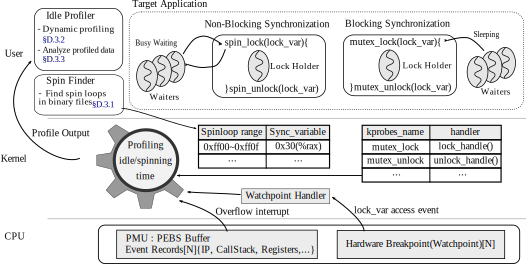
\includegraphics[width=0.90\textwidth]{fig/idleprofiler-dynsync}
\caption{
  The overall architecture of idle profiler, which profiles all kinds
  of synchronization primitives regardless of their running mode
  (kernel or user), types (blocking or non-blocking), and the role of
  tasks (waiter or holder). First, idle proiler analyzes the target
  binary files to find spinning loops that are part of the non-blocking
  synchronization primitives (\autoref{sub:spinfinder}). This is a one time
  job and the extracted spin loop information is cached for future uses.
  Its dynamic profiling mechanism uses the spin loop
  information to profile non-blocking synchronization primitives and
  monitors scheduling boundaries to profile blocking synchronization
  primitives (\autoref{sub:dks}). To reduce runtime overhead,
  it uses hardware performance monitoring features including precise
  event-based sampling (PEBS) and hardware watch-point. The profiled
  data will be used to get an idle graph that represents relations
  among critical sections (\autoref{sub:idlegraph}).
}
\label{f:idleprofiler-overview}
\vspace{-5px}
\end{figure}

\boxbeg
\begin{Challenge}
  In order to provide sufficient information to find scalability
  bottlenecks in a program, the idle profiler should achieve the
  following five goals:
  1) system-wide profiling across the whole software stack including
  user applications and OS kernel 2) for both blocking and non-blocking
  synchronization primitives, 3) that can not only find relations among
  waiting tasks and holding tasks, 4) but also have low profiling overhead
  to find subtle scalability bottlenecks, 5) with no source code modification
  to allow tapping into a real problematic / production environment.
  The challenge lies in achieving all of these goals together
  (for example, low profiling overhead vs. no source code modification).
\end{Challenge}
\boxend

To achieve all of the above goals, we plan to use the following
techniques in the dynamic monitoring of the idle profiler:
1) Instead of profiling each activity of every critical section, we
  will sample only contending ones to reduce profiling overhead;
2) Whenever possible, the profiling activities take place when a
  task is idling. This can effectively hide the profiling overhead;
3) Instead of directly modifying the source code or dynamically instrumenting
  binary files, we will extract necessary information in advance
  (\autoref{sub:spinfinder}) and use a probing mechanism, such as
  \kprobe~\cite{kprobes:doc}, to monitor activities without modifying
  source code.
In the rest of this section, we present in more detail our approach
and preliminary design for both non-blocking and blocking synchronization.

\PP{Non-blocking Synchronization.}
In the dynamic profiling of non-blocking synchronization primitives, we rely on the
spin loop property.
This property states that a non-blocking synchronization primitive has one or more
spin loops, whose exit condition is triggered by another task that is outside
those spin loops.
Thus, a task that spins on those identified spin loops is a waiting task,
whereas the one that triggers the exit condition (i.e., synchronization
variable) is a lock-holding task or a last-arriving task in a spinning
barrier.
\footnote{For brevity, we will simply say a lock holder or lock holding task.}

To detect such spinning tasks with low runtime overhead and without
modifying source code, we will use a hardware performance profiling
feature, Precise Event Based Sampling
(PEBS)~\cite{intel:sys-guide}. In particular, we will track the
exeuction of the conditional branch instructions that are essential in
any loop. We sample the execution of conditional branch using PEBS and
check whether or not its instruction pointer belongs to the pre-identified
spin loops. If so, that running task is a waiting task.

We can find a lock-holding task by finding a task that triggers the
exit condition of a spin loop. When a waiting task is found, we set a
hardware watchpoint~\cite{watchpoint:ols2009} to the
synchronization variable of the spin
loop, which is also pre-identified in~\autoref{sub:spinfinder}. After
setting the watchpoint, any task that writes to the memory address
will be trapped. If the trapped instruction pointer is not the spin
loops (i.e., a task triggers the exit condition of the spin loop), the
running task is a lock holder and is about to release the lock (or the
last task of a spinning barrier just arrived). Thus, we can associate
waiting tasks and holding tasks using the memory address of the
synchronization variable.
There are some design challenges here
since the number of hardware watchpoints is limited (e.g., four in
Intel x86 processors).

\PP{Blocking Synchronization.}
The waiting tasks of a blocking synchronization primitives go to the sleep
state by the task scheduler of the OS kernel. When a holding task releases
a lock, it wakes up one of the waiting tasks to pass over the lock. Thus,
monitoring scheduling boundaries in the kernel is one obvious way to
find critical sections by block synchronization primitives. However, simply
monitoring all scheduling activities will globally inhibit the
performance of the whole system.
For example, in our preliminary evaluation, the \cc{BCC's off-CPU}
analysis, which monitors all scheduling activities, decreased the
throughput of a multi-threaded key-value store, RocksDB, by
70\%. Thus, monitoring all task switch events is not viable to
meet the requirements of low-performance overhead on a production
system. One potential solution is monitoring task switch events only from known
callers using \kprobe. In fact, all user-level blocking
synchronization primitives either use \cc{pthread mutex} that relies on
\cc{futex} system call, or have their own implementation that has a spin
loop composed of a \cc{yield} system call.

%\if 0 Moreover, according to our preliminary experiments described in
%~\autoref{t:prof-overhead}, performance overhead of the existing toos are
%ranging from 25\% to 70\%.
%
%\begin{table}
%\centering
%\scriptsize
%\input{fig/tbl-profile-overhead}
%\caption{Benchmark results of the DB_BENCH(RocksDB)
%	by running 64 threads with various profiling tools.
%\label{t:prof-overhead}
%\end{table}
%\fi
